

\tikzset{every picture/.style={line width=0.75pt}} %set default line width to 0.75pt        

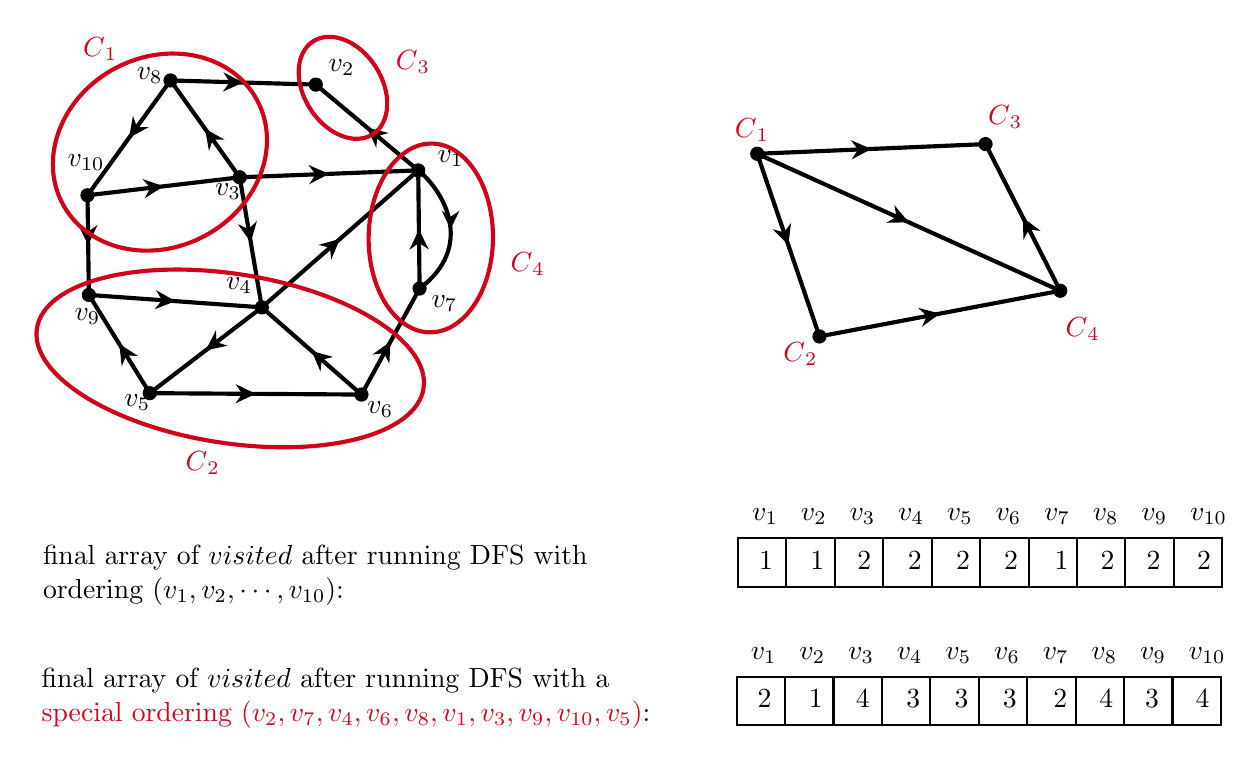
\begin{tikzpicture}[x=0.5pt,y=0.5pt,yscale=-1,xscale=1]
%uncomment if require: \path (0,553); %set diagram left start at 0, and has height of 553

%Flowchart: Connector [id:dp33314190657915177] 
\draw  [fill={rgb, 255:red, 0; green, 0; blue, 0 }  ,fill opacity=1 ] (137,52) .. controls (137,49.58) and (138.96,47.62) .. (141.38,47.62) .. controls (143.79,47.62) and (145.75,49.58) .. (145.75,52) .. controls (145.75,54.42) and (143.79,56.38) .. (141.38,56.38) .. controls (138.96,56.38) and (137,54.42) .. (137,52) -- cycle ;
%Flowchart: Connector [id:dp9493779383807376] 
\draw  [fill={rgb, 255:red, 0; green, 0; blue, 0 }  ,fill opacity=1 ] (242,55) .. controls (242,52.58) and (243.96,50.62) .. (246.38,50.62) .. controls (248.79,50.62) and (250.75,52.58) .. (250.75,55) .. controls (250.75,57.42) and (248.79,59.38) .. (246.38,59.38) .. controls (243.96,59.38) and (242,57.42) .. (242,55) -- cycle ;
%Flowchart: Connector [id:dp6669453073289408] 
\draw  [fill={rgb, 255:red, 0; green, 0; blue, 0 }  ,fill opacity=1 ] (122,278) .. controls (122,275.58) and (123.96,273.62) .. (126.38,273.62) .. controls (128.79,273.62) and (130.75,275.58) .. (130.75,278) .. controls (130.75,280.42) and (128.79,282.38) .. (126.38,282.38) .. controls (123.96,282.38) and (122,280.42) .. (122,278) -- cycle ;
%Flowchart: Connector [id:dp333713085025936] 
\draw  [fill={rgb, 255:red, 0; green, 0; blue, 0 }  ,fill opacity=1 ] (77,135) .. controls (77,132.58) and (78.96,130.62) .. (81.38,130.62) .. controls (83.79,130.62) and (85.75,132.58) .. (85.75,135) .. controls (85.75,137.42) and (83.79,139.38) .. (81.38,139.38) .. controls (78.96,139.38) and (77,137.42) .. (77,135) -- cycle ;
%Flowchart: Connector [id:dp9629725454572109] 
\draw  [fill={rgb, 255:red, 0; green, 0; blue, 0 }  ,fill opacity=1 ] (187,122) .. controls (187,119.58) and (188.96,117.62) .. (191.38,117.62) .. controls (193.79,117.62) and (195.75,119.58) .. (195.75,122) .. controls (195.75,124.42) and (193.79,126.38) .. (191.38,126.38) .. controls (188.96,126.38) and (187,124.42) .. (187,122) -- cycle ;
%Straight Lines [id:da6590518201146447] 
\draw [color={rgb, 255:red, 0; green, 0; blue, 0 }  ,draw opacity=1 ][line width=1.5]    (81.38,135) -- (141.38,52) ;
\draw [shift={(111.38,93.5)}, rotate = 305.86] [fill={rgb, 255:red, 0; green, 0; blue, 0 }  ,fill opacity=1 ][line width=0.08]  [draw opacity=0] (14.56,-6.99) -- (0,0) -- (14.56,6.99) -- (9.67,0) -- cycle    ;
%Straight Lines [id:da1177530387710749] 
\draw [color={rgb, 255:red, 0; green, 0; blue, 0 }  ,draw opacity=1 ][line width=1.5]    (126.38,278) -- (207.38,216) ;
\draw [shift={(166.88,247)}, rotate = 322.57] [fill={rgb, 255:red, 0; green, 0; blue, 0 }  ,fill opacity=1 ][line width=0.08]  [draw opacity=0] (14.56,-6.99) -- (0,0) -- (14.56,6.99) -- (9.67,0) -- cycle    ;
%Straight Lines [id:da8328235451162237] 
\draw [color={rgb, 255:red, 0; green, 0; blue, 0 }  ,draw opacity=1 ][line width=1.5]    (191.38,122) -- (81.38,135) ;
\draw [shift={(136.38,128.5)}, rotate = 173.26] [fill={rgb, 255:red, 0; green, 0; blue, 0 }  ,fill opacity=1 ][line width=0.08]  [draw opacity=0] (14.56,-6.99) -- (0,0) -- (14.56,6.99) -- (9.67,0) -- cycle    ;
%Straight Lines [id:da13491976799128524] 
\draw [color={rgb, 255:red, 0; green, 0; blue, 0 }  ,draw opacity=1 ][line width=1.5]    (126.38,278) -- (82.38,207) ;
\draw [shift={(104.38,242.5)}, rotate = 58.21] [fill={rgb, 255:red, 0; green, 0; blue, 0 }  ,fill opacity=1 ][line width=0.08]  [draw opacity=0] (14.56,-6.99) -- (0,0) -- (14.56,6.99) -- (9.67,0) -- cycle    ;
%Flowchart: Connector [id:dp015404259848177726] 
\draw  [fill={rgb, 255:red, 0; green, 0; blue, 0 }  ,fill opacity=1 ] (275,279) .. controls (275,276.58) and (276.96,274.62) .. (279.38,274.62) .. controls (281.79,274.62) and (283.75,276.58) .. (283.75,279) .. controls (283.75,281.42) and (281.79,283.38) .. (279.38,283.38) .. controls (276.96,283.38) and (275,281.42) .. (275,279) -- cycle ;
%Straight Lines [id:da9050593875476026] 
\draw [color={rgb, 255:red, 0; green, 0; blue, 0 }  ,draw opacity=1 ][line width=1.5]    (279.38,279) -- (321.38,202.38) ;
\draw [shift={(300.38,240.69)}, rotate = 118.73] [fill={rgb, 255:red, 0; green, 0; blue, 0 }  ,fill opacity=1 ][line width=0.08]  [draw opacity=0] (14.56,-6.99) -- (0,0) -- (14.56,6.99) -- (9.67,0) -- cycle    ;
%Straight Lines [id:da6930328339194429] 
\draw [color={rgb, 255:red, 0; green, 0; blue, 0 }  ,draw opacity=1 ][line width=1.5]    (126.38,278) -- (279.38,279) ;
\draw [shift={(202.88,278.5)}, rotate = 180.37] [fill={rgb, 255:red, 0; green, 0; blue, 0 }  ,fill opacity=1 ][line width=0.08]  [draw opacity=0] (14.56,-6.99) -- (0,0) -- (14.56,6.99) -- (9.67,0) -- cycle    ;
%Flowchart: Connector [id:dp8561555389036362] 
\draw  [fill={rgb, 255:red, 0; green, 0; blue, 0 }  ,fill opacity=1 ] (317,202.38) .. controls (317,199.96) and (318.96,198) .. (321.38,198) .. controls (323.79,198) and (325.75,199.96) .. (325.75,202.38) .. controls (325.75,204.79) and (323.79,206.75) .. (321.38,206.75) .. controls (318.96,206.75) and (317,204.79) .. (317,202.38) -- cycle ;
%Straight Lines [id:da4194772983165912] 
\draw [color={rgb, 255:red, 0; green, 0; blue, 0 }  ,draw opacity=1 ][line width=1.5]    (321.38,202.38) -- (320.38,117) ;
\draw [shift={(320.88,159.69)}, rotate = 89.33] [fill={rgb, 255:red, 0; green, 0; blue, 0 }  ,fill opacity=1 ][line width=0.08]  [draw opacity=0] (14.56,-6.99) -- (0,0) -- (14.56,6.99) -- (9.67,0) -- cycle    ;
%Straight Lines [id:da26627336015658065] 
\draw [color={rgb, 255:red, 0; green, 0; blue, 0 }  ,draw opacity=1 ][line width=1.5]    (320.38,117) -- (246.38,55) ;
\draw [shift={(283.38,86)}, rotate = 39.96] [fill={rgb, 255:red, 0; green, 0; blue, 0 }  ,fill opacity=1 ][line width=0.08]  [draw opacity=0] (14.56,-6.99) -- (0,0) -- (14.56,6.99) -- (9.67,0) -- cycle    ;
%Straight Lines [id:da6540321478063363] 
\draw [color={rgb, 255:red, 0; green, 0; blue, 0 }  ,draw opacity=1 ][line width=1.5]    (141.38,52) -- (191.38,122) ;
\draw [shift={(166.38,87)}, rotate = 54.46] [fill={rgb, 255:red, 0; green, 0; blue, 0 }  ,fill opacity=1 ][line width=0.08]  [draw opacity=0] (14.56,-6.99) -- (0,0) -- (14.56,6.99) -- (9.67,0) -- cycle    ;
%Straight Lines [id:da980763773394733] 
\draw [color={rgb, 255:red, 0; green, 0; blue, 0 }  ,draw opacity=1 ][line width=1.5]    (207.38,216) -- (279.38,279) ;
\draw [shift={(243.38,247.5)}, rotate = 41.19] [fill={rgb, 255:red, 0; green, 0; blue, 0 }  ,fill opacity=1 ][line width=0.08]  [draw opacity=0] (14.56,-6.99) -- (0,0) -- (14.56,6.99) -- (9.67,0) -- cycle    ;
%Flowchart: Connector [id:dp884579398191617] 
\draw  [fill={rgb, 255:red, 0; green, 0; blue, 0 }  ,fill opacity=1 ] (203,216) .. controls (203,213.58) and (204.96,211.62) .. (207.38,211.62) .. controls (209.79,211.62) and (211.75,213.58) .. (211.75,216) .. controls (211.75,218.42) and (209.79,220.38) .. (207.38,220.38) .. controls (204.96,220.38) and (203,218.42) .. (203,216) -- cycle ;
%Flowchart: Connector [id:dp3352413725395753] 
\draw  [fill={rgb, 255:red, 0; green, 0; blue, 0 }  ,fill opacity=1 ] (78,207) .. controls (78,204.58) and (79.96,202.62) .. (82.38,202.62) .. controls (84.79,202.62) and (86.75,204.58) .. (86.75,207) .. controls (86.75,209.42) and (84.79,211.38) .. (82.38,211.38) .. controls (79.96,211.38) and (78,209.42) .. (78,207) -- cycle ;
%Flowchart: Connector [id:dp01230167588576514] 
\draw  [fill={rgb, 255:red, 0; green, 0; blue, 0 }  ,fill opacity=1 ] (316,117) .. controls (316,114.58) and (317.96,112.62) .. (320.38,112.62) .. controls (322.79,112.62) and (324.75,114.58) .. (324.75,117) .. controls (324.75,119.42) and (322.79,121.38) .. (320.38,121.38) .. controls (317.96,121.38) and (316,119.42) .. (316,117) -- cycle ;
%Straight Lines [id:da2185567480823013] 
\draw [color={rgb, 255:red, 0; green, 0; blue, 0 }  ,draw opacity=1 ][line width=1.5]    (207.38,216) -- (82.38,207) ;
\draw [shift={(144.88,211.5)}, rotate = 184.12] [fill={rgb, 255:red, 0; green, 0; blue, 0 }  ,fill opacity=1 ][line width=0.08]  [draw opacity=0] (14.56,-6.99) -- (0,0) -- (14.56,6.99) -- (9.67,0) -- cycle    ;
%Curve Lines [id:da3916533808212287] 
\draw [line width=1.5]    (321.38,202.38) .. controls (361.38,172.38) and (339.68,132.52) .. (320.38,117) ;
\draw [shift={(343.77,159.48)}, rotate = 270.05] [fill={rgb, 255:red, 0; green, 0; blue, 0 }  ][line width=0.08]  [draw opacity=0] (13.4,-6.43) -- (0,0) -- (13.4,6.44) -- (8.9,0) -- cycle    ;
%Straight Lines [id:da9071388879776039] 
\draw [color={rgb, 255:red, 0; green, 0; blue, 0 }  ,draw opacity=1 ][line width=1.5]    (207.38,216) -- (320.38,117) ;
\draw [shift={(263.88,166.5)}, rotate = 138.78] [fill={rgb, 255:red, 0; green, 0; blue, 0 }  ,fill opacity=1 ][line width=0.08]  [draw opacity=0] (14.56,-6.99) -- (0,0) -- (14.56,6.99) -- (9.67,0) -- cycle    ;
%Straight Lines [id:da17399207464778044] 
\draw [color={rgb, 255:red, 0; green, 0; blue, 0 }  ,draw opacity=1 ][line width=1.5]    (191.38,122) -- (207.38,216) ;
\draw [shift={(199.38,169)}, rotate = 260.34] [fill={rgb, 255:red, 0; green, 0; blue, 0 }  ,fill opacity=1 ][line width=0.08]  [draw opacity=0] (14.56,-6.99) -- (0,0) -- (14.56,6.99) -- (9.67,0) -- cycle    ;
%Straight Lines [id:da8016859457087312] 
\draw [color={rgb, 255:red, 0; green, 0; blue, 0 }  ,draw opacity=1 ][line width=1.5]    (81.38,135) -- (82.38,207) ;
\draw [shift={(81.88,171)}, rotate = 269.2] [fill={rgb, 255:red, 0; green, 0; blue, 0 }  ,fill opacity=1 ][line width=0.08]  [draw opacity=0] (14.56,-6.99) -- (0,0) -- (14.56,6.99) -- (9.67,0) -- cycle    ;
%Straight Lines [id:da8138783684306082] 
\draw [color={rgb, 255:red, 0; green, 0; blue, 0 }  ,draw opacity=1 ][line width=1.5]    (191.38,122) -- (320.38,117) ;
\draw [shift={(255.88,119.5)}, rotate = 177.78] [fill={rgb, 255:red, 0; green, 0; blue, 0 }  ,fill opacity=1 ][line width=0.08]  [draw opacity=0] (14.56,-6.99) -- (0,0) -- (14.56,6.99) -- (9.67,0) -- cycle    ;
%Straight Lines [id:da24392431611835252] 
\draw [color={rgb, 255:red, 0; green, 0; blue, 0 }  ,draw opacity=1 ][line width=1.5]    (141.38,52) -- (246.38,55) ;
\draw [shift={(193.88,53.5)}, rotate = 181.64] [fill={rgb, 255:red, 0; green, 0; blue, 0 }  ,fill opacity=1 ][line width=0.08]  [draw opacity=0] (14.56,-6.99) -- (0,0) -- (14.56,6.99) -- (9.67,0) -- cycle    ;
%Shape: Ellipse [id:dp837267975011143] 
\draw  [color={rgb, 255:red, 208; green, 2; blue, 27 }  ,draw opacity=1 ][line width=1.5]  (63.39,141.12) .. controls (45.61,107.62) and (62.68,63.75) .. (101.52,43.13) .. controls (140.37,22.52) and (186.27,32.96) .. (204.05,66.45) .. controls (221.83,99.95) and (204.76,143.82) .. (165.91,164.44) .. controls (127.07,185.06) and (81.17,174.61) .. (63.39,141.12) -- cycle ;
%Shape: Ellipse [id:dp6301102730017264] 
\draw  [color={rgb, 255:red, 208; green, 2; blue, 27 }  ,draw opacity=1 ][line width=1.5]  (44.82,231.18) .. controls (50.01,197.81) and (116.75,180.47) .. (193.91,192.46) .. controls (271.06,204.44) and (329.4,241.21) .. (324.22,274.58) .. controls (319.04,307.95) and (252.29,325.29) .. (175.14,313.3) .. controls (97.98,301.32) and (39.64,264.55) .. (44.82,231.18) -- cycle ;
%Shape: Ellipse [id:dp9534249176688527] 
\draw  [color={rgb, 255:red, 208; green, 2; blue, 27 }  ,draw opacity=1 ][line width=1.5]  (330.2,97.61) .. controls (355.02,97.88) and (374.8,128.63) .. (374.4,166.31) .. controls (374,203.98) and (353.56,234.31) .. (328.75,234.04) .. controls (303.94,233.78) and (284.15,203.02) .. (284.55,165.35) .. controls (284.96,127.68) and (305.39,97.35) .. (330.2,97.61) -- cycle ;
%Shape: Ellipse [id:dp8449632734349601] 
\draw  [color={rgb, 255:red, 208; green, 2; blue, 27 }  ,draw opacity=1 ][line width=1.5]  (244.45,23.74) .. controls (257.53,15.36) and (277.77,23.6) .. (289.66,42.15) .. controls (301.55,60.71) and (300.58,82.54) .. (287.5,90.92) .. controls (274.42,99.3) and (254.19,91.05) .. (242.3,72.5) .. controls (230.41,53.95) and (231.38,32.12) .. (244.45,23.74) -- cycle ;
%Flowchart: Connector [id:dp603695290762529] 
\draw  [fill={rgb, 255:red, 0; green, 0; blue, 0 }  ,fill opacity=1 ] (606,237) .. controls (606,234.58) and (607.96,232.62) .. (610.38,232.62) .. controls (612.79,232.62) and (614.75,234.58) .. (614.75,237) .. controls (614.75,239.42) and (612.79,241.38) .. (610.38,241.38) .. controls (607.96,241.38) and (606,239.42) .. (606,237) -- cycle ;
%Straight Lines [id:da27444933364712354] 
\draw [color={rgb, 255:red, 0; green, 0; blue, 0 }  ,draw opacity=1 ][line width=1.5]    (784.38,204) -- (565.38,105) ;
\draw [shift={(674.88,154.5)}, rotate = 204.33] [fill={rgb, 255:red, 0; green, 0; blue, 0 }  ,fill opacity=1 ][line width=0.08]  [draw opacity=0] (14.56,-6.99) -- (0,0) -- (14.56,6.99) -- (9.67,0) -- cycle    ;
%Straight Lines [id:da6238918789957093] 
\draw [color={rgb, 255:red, 0; green, 0; blue, 0 }  ,draw opacity=1 ][line width=1.5]    (784.38,204) -- (730.38,98) ;
\draw [shift={(757.38,151)}, rotate = 63] [fill={rgb, 255:red, 0; green, 0; blue, 0 }  ,fill opacity=1 ][line width=0.08]  [draw opacity=0] (14.56,-6.99) -- (0,0) -- (14.56,6.99) -- (9.67,0) -- cycle    ;
%Flowchart: Connector [id:dp07658274147850641] 
\draw  [fill={rgb, 255:red, 0; green, 0; blue, 0 }  ,fill opacity=1 ] (726,98) .. controls (726,95.58) and (727.96,93.62) .. (730.38,93.62) .. controls (732.79,93.62) and (734.75,95.58) .. (734.75,98) .. controls (734.75,100.42) and (732.79,102.38) .. (730.38,102.38) .. controls (727.96,102.38) and (726,100.42) .. (726,98) -- cycle ;
%Flowchart: Connector [id:dp6792415791877835] 
\draw  [fill={rgb, 255:red, 0; green, 0; blue, 0 }  ,fill opacity=1 ] (561,105) .. controls (561,102.58) and (562.96,100.62) .. (565.38,100.62) .. controls (567.79,100.62) and (569.75,102.58) .. (569.75,105) .. controls (569.75,107.42) and (567.79,109.38) .. (565.38,109.38) .. controls (562.96,109.38) and (561,107.42) .. (561,105) -- cycle ;
%Straight Lines [id:da6954252151831065] 
\draw [color={rgb, 255:red, 0; green, 0; blue, 0 }  ,draw opacity=1 ][line width=1.5]    (610.38,237) -- (565.38,105) ;
\draw [shift={(587.88,171)}, rotate = 251.18] [fill={rgb, 255:red, 0; green, 0; blue, 0 }  ,fill opacity=1 ][line width=0.08]  [draw opacity=0] (14.56,-6.99) -- (0,0) -- (14.56,6.99) -- (9.67,0) -- cycle    ;
%Straight Lines [id:da21094314981608042] 
\draw [color={rgb, 255:red, 0; green, 0; blue, 0 }  ,draw opacity=1 ][line width=1.5]    (565.38,105) -- (730.38,98) ;
\draw [shift={(647.88,101.5)}, rotate = 177.57] [fill={rgb, 255:red, 0; green, 0; blue, 0 }  ,fill opacity=1 ][line width=0.08]  [draw opacity=0] (14.56,-6.99) -- (0,0) -- (14.56,6.99) -- (9.67,0) -- cycle    ;
%Flowchart: Connector [id:dp8786817451944372] 
\draw  [fill={rgb, 255:red, 0; green, 0; blue, 0 }  ,fill opacity=1 ] (780,204) .. controls (780,201.58) and (781.96,199.62) .. (784.38,199.62) .. controls (786.79,199.62) and (788.75,201.58) .. (788.75,204) .. controls (788.75,206.42) and (786.79,208.38) .. (784.38,208.38) .. controls (781.96,208.38) and (780,206.42) .. (780,204) -- cycle ;
%Straight Lines [id:da6613494332963039] 
\draw [color={rgb, 255:red, 0; green, 0; blue, 0 }  ,draw opacity=1 ][line width=1.5]    (784.38,204) -- (610.38,237) ;
\draw [shift={(697.38,220.5)}, rotate = 169.26] [fill={rgb, 255:red, 0; green, 0; blue, 0 }  ,fill opacity=1 ][line width=0.08]  [draw opacity=0] (14.56,-6.99) -- (0,0) -- (14.56,6.99) -- (9.67,0) -- cycle    ;
%Shape: Grid [id:dp7216183755073775] 
\draw  [draw opacity=0] (551.5,382.87) -- (901.5,382.87) -- (901.5,417.87) -- (551.5,417.87) -- cycle ; \draw   (586.5,382.87) -- (586.5,417.87)(621.5,382.87) -- (621.5,417.87)(656.5,382.87) -- (656.5,417.87)(691.5,382.87) -- (691.5,417.87)(726.5,382.87) -- (726.5,417.87)(761.5,382.87) -- (761.5,417.87)(796.5,382.87) -- (796.5,417.87)(831.5,382.87) -- (831.5,417.87)(866.5,382.87) -- (866.5,417.87) ; \draw    ; \draw   (551.5,382.87) -- (901.5,382.87) -- (901.5,417.87) -- (551.5,417.87) -- cycle ;
%Shape: Grid [id:dp08811438988655107] 
\draw  [draw opacity=0] (550.5,482.87) -- (900.5,482.87) -- (900.5,517.87) -- (550.5,517.87) -- cycle ; \draw   (585.5,482.87) -- (585.5,517.87)(620.5,482.87) -- (620.5,517.87)(655.5,482.87) -- (655.5,517.87)(690.5,482.87) -- (690.5,517.87)(725.5,482.87) -- (725.5,517.87)(760.5,482.87) -- (760.5,517.87)(795.5,482.87) -- (795.5,517.87)(830.5,482.87) -- (830.5,517.87)(865.5,482.87) -- (865.5,517.87) ; \draw    ; \draw   (550.5,482.87) -- (900.5,482.87) -- (900.5,517.87) -- (550.5,517.87) -- cycle ;

% Text Node
\draw (332.2,100.61) node [anchor=north west][inner sep=0.75pt]   [align=left] {$\displaystyle v_{1}$};
% Text Node
\draw (171.38,124.38) node [anchor=north west][inner sep=0.75pt]   [align=left] {$\displaystyle v_{3}$};
% Text Node
\draw (105.75,277) node [anchor=north west][inner sep=0.75pt]   [align=left] {$\displaystyle v_{5}$};
% Text Node
\draw (179.38,192.38) node [anchor=north west][inner sep=0.75pt]   [align=left] {$\displaystyle v_{4}$};
% Text Node
\draw (253.38,34.38) node [anchor=north west][inner sep=0.75pt]   [align=left] {$\displaystyle v_{2}$};
% Text Node
\draw (69.75,214.35) node [anchor=north west][inner sep=0.75pt]   [align=left] {$\displaystyle v_{9}$};
% Text Node
\draw (327.75,205.38) node [anchor=north west][inner sep=0.75pt]   [align=left] {$\displaystyle v_{7}$};
% Text Node
\draw (281.38,282) node [anchor=north west][inner sep=0.75pt]   [align=left] {$\displaystyle v_{6}$};
% Text Node
\draw (114.75,40.35) node [anchor=north west][inner sep=0.75pt]   [align=left] {$\displaystyle v_{8}$};
% Text Node
\draw (64.75,103.35) node [anchor=north west][inner sep=0.75pt]   [align=left] {$\displaystyle v_{10}$};
% Text Node
\draw (76,19) node [anchor=north west][inner sep=0.75pt]   [align=left] {$\displaystyle \textcolor[rgb]{0.82,0.01,0.11}{C}\textcolor[rgb]{0.82,0.01,0.11}{_{1}}$};
% Text Node
\draw (150,318) node [anchor=north west][inner sep=0.75pt]   [align=left] {$\displaystyle \textcolor[rgb]{0.82,0.01,0.11}{C}\textcolor[rgb]{0.82,0.01,0.11}{_{2}}$};
% Text Node
\draw (385,174) node [anchor=north west][inner sep=0.75pt]   [align=left] {$\displaystyle \textcolor[rgb]{0.82,0.01,0.11}{C}\textcolor[rgb]{0.82,0.01,0.11}{_{4}}$};
% Text Node
\draw (302,28) node [anchor=north west][inner sep=0.75pt]   [align=left] {$\displaystyle \textcolor[rgb]{0.82,0.01,0.11}{C}\textcolor[rgb]{0.82,0.01,0.11}{_{3}}$};
% Text Node
\draw (582,239) node [anchor=north west][inner sep=0.75pt]   [align=left] {$\displaystyle \textcolor[rgb]{0.82,0.01,0.11}{C}\textcolor[rgb]{0.82,0.01,0.11}{_{2}}$};
% Text Node
\draw (786,221) node [anchor=north west][inner sep=0.75pt]   [align=left] {$\displaystyle \textcolor[rgb]{0.82,0.01,0.11}{C}\textcolor[rgb]{0.82,0.01,0.11}{_{4}}$};
% Text Node
\draw (547,77) node [anchor=north west][inner sep=0.75pt]   [align=left] {$\displaystyle \textcolor[rgb]{0.82,0.01,0.11}{C}\textcolor[rgb]{0.82,0.01,0.11}{_{1}}$};
% Text Node
\draw (730,68) node [anchor=north west][inner sep=0.75pt]   [align=left] {$\displaystyle \textcolor[rgb]{0.82,0.01,0.11}{C}\textcolor[rgb]{0.82,0.01,0.11}{_{3}}$};
% Text Node
\draw (47,385.93) node [anchor=north west][inner sep=0.75pt]   [align=left] {final array of $\displaystyle visited$ after running DFS with\\ordering $\displaystyle ( v_{1} ,v_{2} ,\cdots ,v_{10})$:};
% Text Node
\draw (672,390.37) node [anchor=north west][inner sep=0.75pt]   [align=left] {$\displaystyle 2$};
% Text Node
\draw (706.83,390.37) node [anchor=north west][inner sep=0.75pt]   [align=left] {$\displaystyle 2$};
% Text Node
\draw (741.66,390.37) node [anchor=north west][inner sep=0.75pt]   [align=left] {$\displaystyle 2$};
% Text Node
\draw (844.49,390.37) node [anchor=north west][inner sep=0.75pt]   [align=left] {$\displaystyle 2$};
% Text Node
\draw (811.32,390.37) node [anchor=north west][inner sep=0.75pt]   [align=left] {$\displaystyle 2$};
% Text Node
\draw (778.15,390.37) node [anchor=north west][inner sep=0.75pt]   [align=left] {$\displaystyle 1$};
% Text Node
\draw (881,390.37) node [anchor=north west][inner sep=0.75pt]   [align=left] {$\displaystyle 2$};
% Text Node
\draw (564.49,390.37) node [anchor=north west][inner sep=0.75pt]   [align=left] {$\displaystyle 1$};
% Text Node
\draw (601.49,390.37) node [anchor=north west][inner sep=0.75pt]   [align=left] {$\displaystyle 1$};
% Text Node
\draw (635.49,390.37) node [anchor=north west][inner sep=0.75pt]   [align=left] {$\displaystyle 2$};
% Text Node
\draw (665,359.37) node [anchor=north west][inner sep=0.75pt]   [align=left] {$\displaystyle v_{4}$};
% Text Node
\draw (700.17,359.37) node [anchor=north west][inner sep=0.75pt]   [align=left] {$\displaystyle v_{5}$};
% Text Node
\draw (735.34,359.37) node [anchor=north west][inner sep=0.75pt]   [align=left] {$\displaystyle v_{6}$};
% Text Node
\draw (840.85,359.37) node [anchor=north west][inner sep=0.75pt]   [align=left] {$\displaystyle v_{9}$};
% Text Node
\draw (805.68,359.37) node [anchor=north west][inner sep=0.75pt]   [align=left] {$\displaystyle v_{8}$};
% Text Node
\draw (770.51,359.37) node [anchor=north west][inner sep=0.75pt]   [align=left] {$\displaystyle v_{7}$};
% Text Node
\draw (876,359.37) node [anchor=north west][inner sep=0.75pt]   [align=left] {$\displaystyle v_{10}$};
% Text Node
\draw (559.49,359.37) node [anchor=north west][inner sep=0.75pt]   [align=left] {$\displaystyle v_{1}$};
% Text Node
\draw (594.66,359.37) node [anchor=north west][inner sep=0.75pt]   [align=left] {$\displaystyle v_{2}$};
% Text Node
\draw (629.83,359.37) node [anchor=north west][inner sep=0.75pt]   [align=left] {$\displaystyle v_{3}$};
% Text Node
\draw (46,474.93) node [anchor=north west][inner sep=0.75pt]   [align=left] {final array of $\displaystyle visited$ after running DFS with a \\\textcolor[rgb]{0.82,0.01,0.11}{special ordering }$\displaystyle \textcolor[rgb]{0.82,0.01,0.11}{( v_{2} ,v_{7} ,v_{4} ,v_{6} ,v_{8} ,v_{1} ,v_{3} ,v_{9} ,v_{10} ,v_{5})}$:};
% Text Node
\draw (671,490.37) node [anchor=north west][inner sep=0.75pt]   [align=left] {$\displaystyle 3$};
% Text Node
\draw (705.83,490.37) node [anchor=north west][inner sep=0.75pt]   [align=left] {$\displaystyle 3$};
% Text Node
\draw (740.66,490.37) node [anchor=north west][inner sep=0.75pt]   [align=left] {$\displaystyle 3$};
% Text Node
\draw (843.49,490.37) node [anchor=north west][inner sep=0.75pt]   [align=left] {$\displaystyle 3$};
% Text Node
\draw (810.32,490.37) node [anchor=north west][inner sep=0.75pt]   [align=left] {$\displaystyle 4$};
% Text Node
\draw (777.15,490.37) node [anchor=north west][inner sep=0.75pt]   [align=left] {$\displaystyle 2$};
% Text Node
\draw (880,490.37) node [anchor=north west][inner sep=0.75pt]   [align=left] {$\displaystyle 4$};
% Text Node
\draw (563.49,490.37) node [anchor=north west][inner sep=0.75pt]   [align=left] {$\displaystyle 2$};
% Text Node
\draw (600.49,490.37) node [anchor=north west][inner sep=0.75pt]   [align=left] {$\displaystyle 1$};
% Text Node
\draw (634.49,490.37) node [anchor=north west][inner sep=0.75pt]   [align=left] {$\displaystyle 4$};
% Text Node
\draw (664,459.37) node [anchor=north west][inner sep=0.75pt]   [align=left] {$\displaystyle v_{4}$};
% Text Node
\draw (699.17,459.37) node [anchor=north west][inner sep=0.75pt]   [align=left] {$\displaystyle v_{5}$};
% Text Node
\draw (734.34,459.37) node [anchor=north west][inner sep=0.75pt]   [align=left] {$\displaystyle v_{6}$};
% Text Node
\draw (839.85,459.37) node [anchor=north west][inner sep=0.75pt]   [align=left] {$\displaystyle v_{9}$};
% Text Node
\draw (804.68,459.37) node [anchor=north west][inner sep=0.75pt]   [align=left] {$\displaystyle v_{8}$};
% Text Node
\draw (769.51,459.37) node [anchor=north west][inner sep=0.75pt]   [align=left] {$\displaystyle v_{7}$};
% Text Node
\draw (875,459.37) node [anchor=north west][inner sep=0.75pt]   [align=left] {$\displaystyle v_{10}$};
% Text Node
\draw (558.49,459.37) node [anchor=north west][inner sep=0.75pt]   [align=left] {$\displaystyle v_{1}$};
% Text Node
\draw (593.66,459.37) node [anchor=north west][inner sep=0.75pt]   [align=left] {$\displaystyle v_{2}$};
% Text Node
\draw (628.83,459.37) node [anchor=north west][inner sep=0.75pt]   [align=left] {$\displaystyle v_{3}$};


\end{tikzpicture}

